% Global document settings
\documentclass[10pt]{article}  % This specifies the type of document to be created and the default font size

% Packages
\usepackage{tgtermes}  % Loads the TeX Gyre Termes font
\usepackage{graphicx}  % Enhances LaTeX's built-in graphics features
% \usepackage{background} % Creates background images on pages
\usepackage{natbib}  % A package for bibliographies and citations
\usepackage{authblk}  % For author and affiliation management
\usepackage{tocloft}  % Controls the typographic design of table of contents, list of figures and list of tables
\usepackage{xcolor}  % Provides easy driver-independent access to colors
\usepackage{siunitx}  % A comprehensive (SI) units package
\usepackage{setspace}  % Controls line spacing
\usepackage{listings}  % Typeset programming code within the document
\usepackage[T1]{fontenc}  % Choice of font encodings
\usepackage[nottoc]{tocbibind}  % Adds entries for lof, lot, bibliography etc. to the table of contents
\usepackage[breaklinks,linktocpage]{hyperref}  % Creates hyperlinks in your document
\usepackage[font=small,skip=7pt,labelfont=bf]{caption}  % Customizing captions in floating environments

% Custom colours
% Here we define custom colors to use within code listings
\definecolor{codegreen}{rgb}{0,0.5,0}
\definecolor{codegray}{rgb}{0.4,0.4,0.4}
\definecolor{codepurple}{rgb}{0.58,0,0.82}
\definecolor{backcolour}{rgb}{0.96,0.96,0.96}

\lstdefinelanguage{JavaScript}{
  keywords={break, case, catch, continue, debugger, default, delete, do, else, finally, for, function, if, in, instanceof, new, return, switch, this, throw, try, typeof, var, void, while, with},
  morecomment=[l]{//},
  morecomment=[s]{/*}{*/},
  morestring=[b]',
  morestring=[b]",
  sensitive=true
}

% Listing styles
% This defines a custom style for code listings
\lstdefinestyle{mystyle}{
  % ... various style settings ...
  backgroundcolor=\color{backcolour},
  commentstyle=\color{codegreen},
  keywordstyle=\color{purple},
  numberstyle=\tiny\color{codegray},
  stringstyle=\color{codepurple},
  basicstyle=\ttfamily\footnotesize,
  breakatwhitespace=false,
  breaklines=true,
  captionpos=b,
  framextopmargin=6pt,
  framexbottommargin=6pt,
  frame=tb,
  framerule=0pt,
  keepspaces=true,
  numbers=left,
  numbersep=5pt,
  showspaces=false,
  showstringspaces=true,
  showtabs=false,
  tabsize=2
  }
  \lstset{style=mystyle}  % Apply the custom style to future listings

  % Custom commands
% Here we modify some LaTeX default commands
\renewcommand\cftsecafterpnum{\vskip8pt}  % Add a vertical space after section numbers in ToC
\renewcommand{\lstlistlistingname}{List of \lstlistingname s}  % Changes the title of the list of listings
\renewcommand{\bibsection}{\section*{Bibliography}}  % Changes the bibliography section name
\renewcommand{\contentsname}{Table of Contents}  % Changes the title of the table of contents
\renewcommand{\cftsecleader}{\cftdotfill{\cftdotsep}}  % Changes the leader between section names and page numbers in ToC
\newcommand{\floatcaption}[2]{\caption[#1.]{#1~#2.}}



% Custom settings
\captionsetup{justification=centering}  % All captions will be centered
% \backgroundsetup{contents=Preprint, opacity=0.25, color=gray} % Adds a watermark to the document
\PassOptionsToPackage{hyphens}{url}  % Allow hyphenated URLs
\urlstyle{same}  % The same font that is being used in the text will be used for URLs
\def\Urlmuskip{0mu}  % No additional space between characters in a URL
\def\UrlBreaks{\do\/\do-}  % URL line breaks at / and -
\hypersetup{  % Setup for the hyperref package
    colorlinks = true,
    urlcolor = blue,
    linkcolor = blue,
    citecolor = blue,
  breaklinks=true,
  pdfpagemode=UseOutlines,
  bookmarksopen=true,
  bookmarksopenlevel=2,
  bookmarksnumbered=true
  }

  \title{\textbf{WebAssembly and the \linebreak  Wizards of Hogwarts}}  % Document title
  \author[1]{Daniel Burger}  % Author name
  \affil[1]{\textbf{Middlesex University London\thanks{In collaboration with SAE Institute Zürich.}}}  % Author affiliation
  \affil[ ]{\href{mailto:public@danielburger.online}{public@danielburger.online}}  % Author email
  \date{\textit{7. November 2020}} % Document date

% Start of the document content
\begin{document}
\pagenumbering{roman}
\counterwithin{lstlisting}{section}
\counterwithin{figure}{section}
\counterwithin{table}{section}
\setlength{\footskip}{65pt} % This command sets the distance between the bottom of the text body and the footer

\maketitle  % This command prints the title, author, and date as defined earlier

\thispagestyle{empty}  % This command sets the style of the current page to empty, removing headers and footers

\begin{sloppypar}  % The sloppypar environment adjusts the spaces between words such that each line fits into the text width
  \begin{abstract}  % Start of the abstract
    There is a new kind in the web development hood: WebAssembly. It is fast, portable, supported by the big players and should allow making the world wide web the biggest software platform in existence. It doesn’t matter if you are an experienced software architect or a frontend developer—everyone will be able to profit from WebAssembly’s existence.

    In this essay, we will look at what WebAssembly is, how it works and how it works alongside its sibling JavaScript.
  \end{abstract}  % End of the abstract

  \pagebreak  % This command inserts a page break

  \pagenumbering{Roman}  % This command changes the page numbering to uppercase Roman numerals

  \tableofcontents  % This command prints the table of contents

  \pagebreak  % Page break

  \listoffigures  % This command prints the list of figures

  \pagebreak  % Page break

  \listoftables  % This command prints the list of tables

  \pagebreak  % Page break

  \addcontentsline{toc}{section}{\lstlistlistingname}  % This command adds the list of listings to the table of contents
  \lstlistoflistings  % This command prints the list of code listings

  \pagebreak  % Page break

  % \doublespacing  % This command changes the line spacing to double

  \pagenumbering{arabic}  % This command changes the page numbering back to Arabic numerals

  \section{Introduction}
  \label{sec:introduction}

  On the 17th of June 2015, Brendan Eich—the inventor of JavaScript—and the teams behind Mozilla, Chromium, Edge and WebKit presented a new browser standard: \mbox{WebAssembly}, a portable and highly efficient byte-code compilation target for high-level languages such as C++ and Rust \citep{eich_asmjs_2015}.

  However, what does this mean? What is the reason that WebAssembly should exist in the first place? Should JavaScript developers be worried now? And what do the wizards of Hogwarts have to do with it?

  \subsection{Web Development Back Then}
  \label{sec:back-then}

  Back in the day when you could call yourself web developer because you only understood HTML, web development itself was a rather interactionless and static field of business. Netscape Communications, a pivotal company in the development of the modern web and the creator of the Netscape Browser (shown in \autoref{fig:netscape}), quickly recognised that websites of the time lacked interactivity and dynamism. They wanted the web to be a new form of a distributed operating system rather than just a simple HTML document-accessing application on your computer \citep{cassel_brendan_2018}.

  \begin{figure}[ht]
    \centering
    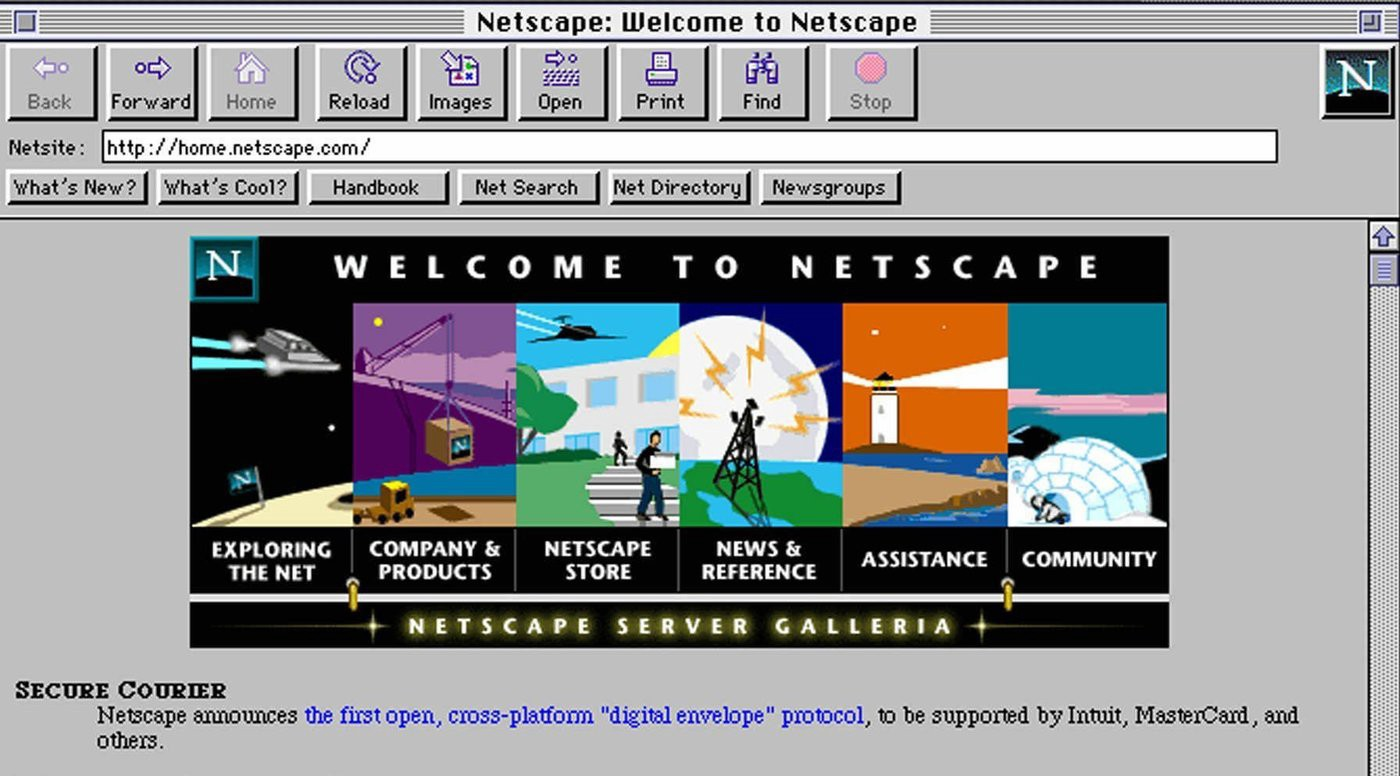
\includegraphics[width=\textwidth]{figures/netscape.jpg}
    \floatcaption{Screenshot of the Netscape browser and start-page}{\citep{npr_home_nodate}}
    \label{fig:netscape}
  \end{figure}

  Marc Andreessen, who was the founder of Netscape Communications, proposed that HTML needed some kind of “scripting language” that was approachable; something you could glue directly into the markup. A language that is easy to use by newbie programmers who didn’t want to handle compiler errors or strictly-typed syntax.

  That was the reason they hired the experienced programming language and network code developer Brendan Eich. Brendan’s first task was the nearly unachievable goal of creating such a scripting language for the web—due in 10 days. They (later) called it: JavaScript \citep{severance_javascript_2012}.

  \subsection{JavaScript’s Destiny}
  \label{sec:javascript-destiny}

  I don’t need to dig too deep into the history of the web to show you one crucial pain point of today’s web technology standards: JavaScript is a scripting language for the browser to interpret. I repeat it: JavaScript is a scripting language for the browser to interpret—not some fancy multi-paradigm system programming language that focuses on speed, security or code maintainability. It was supposed and designed to be an easy-to-understand dynamically-typed scripting language to give your website some cool DOM manipulations and decorative animations.

  Nevertheless, see what happened:

  \begin{quote}
    \emph{``Any application that can be written in JavaScript, will eventually be written in JavaScript.'' \citep{atwood_principle_2007}}
  \end{quote}

  A quote by Jeff Atwood (co-founder of Stack Exchange) that is popularly referred to as Atwood’s Law. Ever since frameworks like Node.js or React Native became widely used, JavaScript’s possibilities already crossed the border of just living on the client-side inside of a browser. It’s nearly everywhere.

  Also, Node.js’ NPM package manager is currently the most prominent and most active package registry platform ever created. As an example: From May 10th to May 17th of 2018, JavaScript developers downloaded 5.2 billion Node.js packages from the NPM registry, setting a new record \citep{inc_how_2018}

  \begin{figure}[ht]
    \centering
    \frame{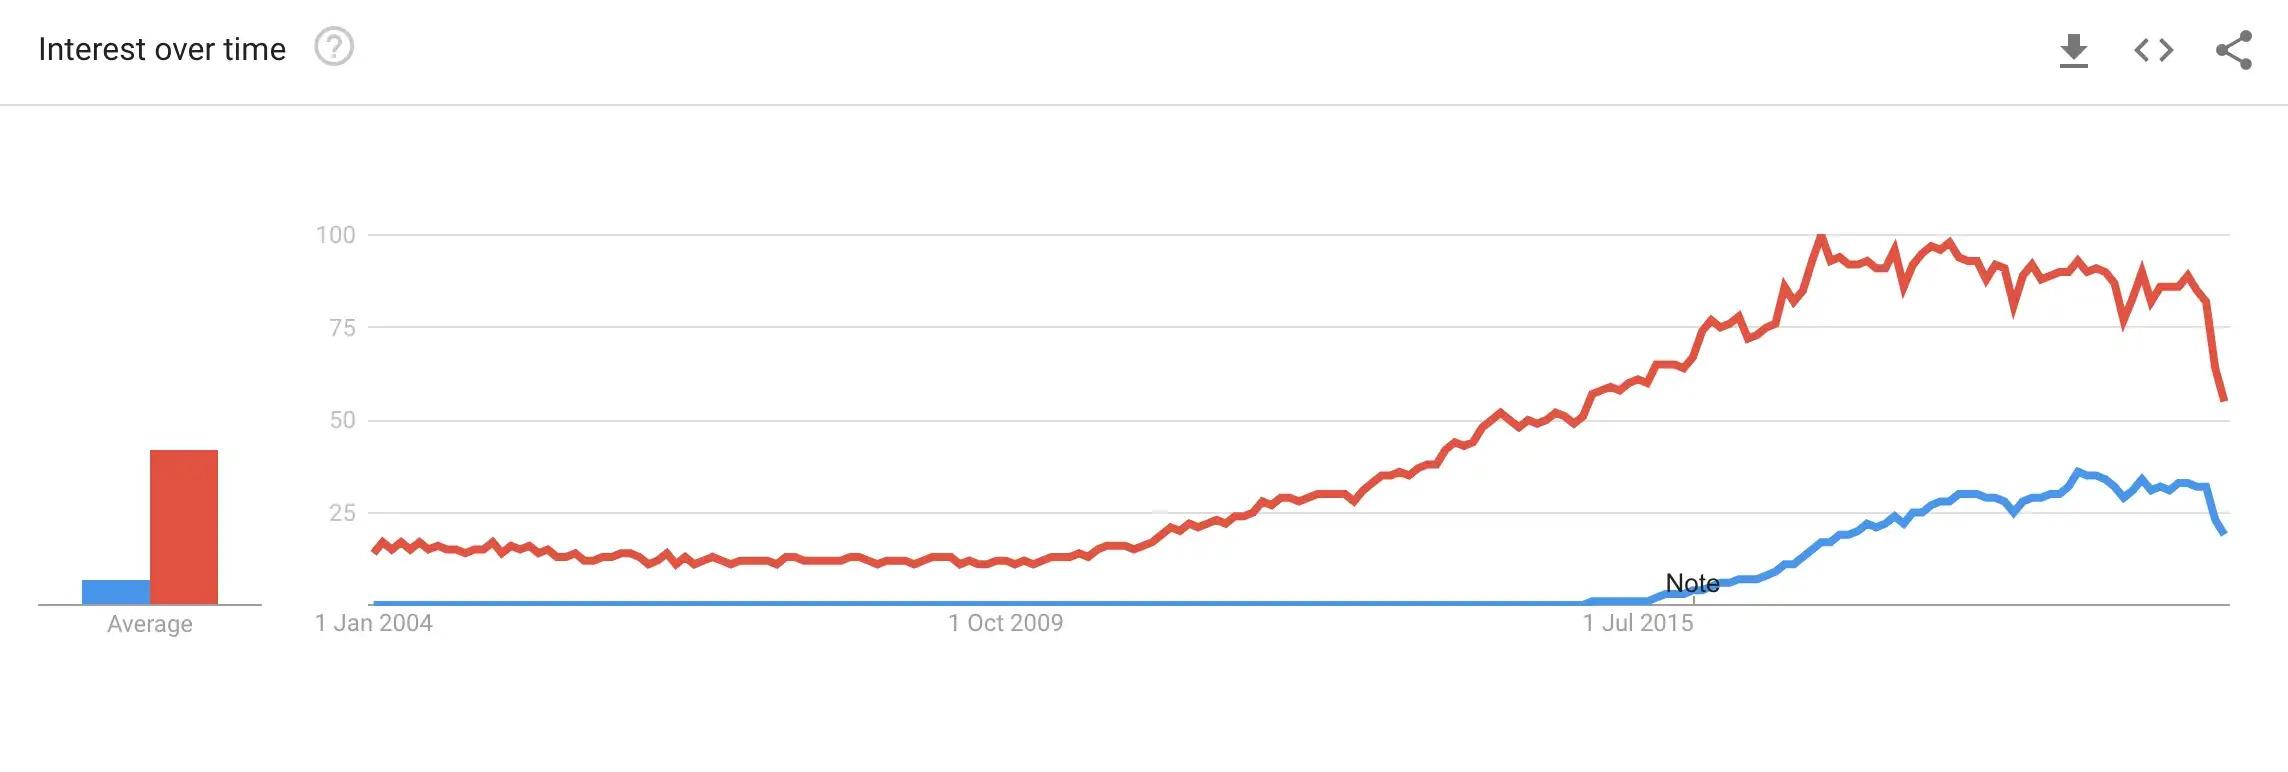
\includegraphics[width=\textwidth]{figures/google-trends.jpg}}
    \floatcaption{Google Trends curve about Node.js and React Native}{\citep{google_google_nodate}}
    \label{fig:atwood-law}
  \end{figure}

  \subsection{Treacherous Atwood’s Law}
  \label{sec:atwood-law}

  There are thousands of courses, books and tutorials on how to learn JavaScript. Every computer-related school now or then teaches JavaScript. Nearly everyone could be able to learn it anywhere with a minimum amount of effort. If you search for “Learn JavaScript” on Google, you’ll get \num{2220000000} search results. In comparison: When you search “Learn Java” you’ll get \num{305000000} results.

  Though, is that a good thing? Is an originally lightweight scripting language capable of ruling the world of computational web development? My opinion: No, it’s not, and I believe there won’t be such a bright future for JavaScript as nearly everybody claims. Let me explain it with a Harry Potter analogy:

  \subsection{Muggles Entering Hogwarts}
  \label{sec:muggles}

  Do you know how it feels to watch frontend developers call themselves “full-stack software developer” after they’ve simply learned Node.js? It feels like Muggles entering Hogwarts—a school full of wizards. Only that in our case these wizards are trained software engineers and computer scientists. These are the people who learn all the hardcore-implemented algorithms and compilers, programming languages and operating systems. They know precisely how to build software \citep{might_what_2011}. Do frontend developers know how to write actual software? I’d say we better don’t talk about it.

  Muggles aren’t invited to Hogwarts because they have no magical ability. Frontend developers weren’t “invited” for software engineering too because they couldn’t even do something with the languages they knew. Nevertheless, now—thanks to all the cross-platform JavaScript runtimes—they’re suddenly here to do some magic. But imagine, what if the wizards of Hogwarts, our beloved software engineers and computer scientists, would be able to perform magic in the real world—or our case: the frontend? What would happen? What could go wrong?

  \section{WebAssembly Says Hello World}
  \label{sec:hello-world}

  WebAssembly is the new player in the web development industry. It’s fast, small, non-readable and not even a real programming language. Yes, you heard that right. You literally can’t code in WebAssembly \citep{rourke_learn_2018}. So I may hear you asking: Why should we all be excited about it? Well, as mentioned earlier, it’s a compilation byte-format target for high-level languages.

  \begin{figure}[ht]
    \centering
    \frame{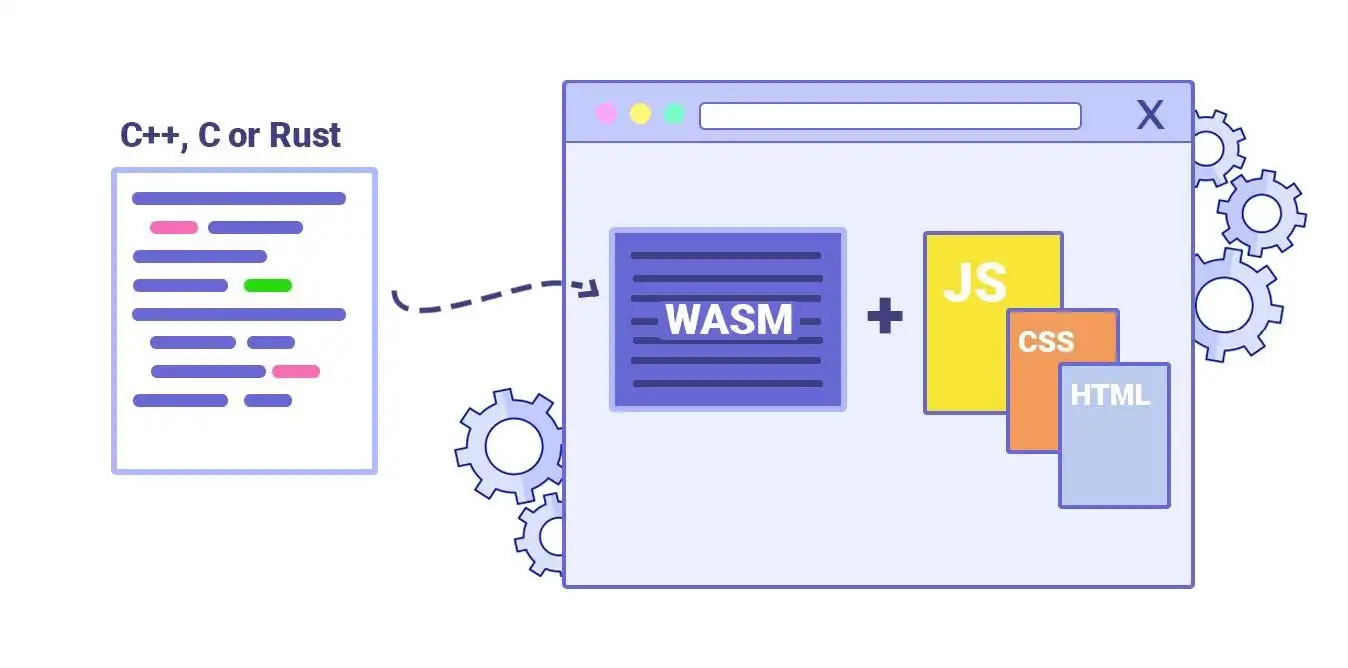
\includegraphics[width=\textwidth]{figures/wasm.jpg}}
    \floatcaption{Illustration of how WebAssembly modules are being delivered to the browser}{\citep{logrocket_logrocket_nodate}}
    \label{fig:wasm}
  \end{figure}

  You write your code in such a high-level language like C or C++ and compile it down to WebAssembly. The magic trick: It works in the browser, and it’s super fast—sometimes about 5 to 20 times faster than JavaScript \citep{aboukhalil_how_2019}.

  \section{WebAssembly in a Nutshell}
  \label{sec:wasm-in-a-nutshell}

  Enough with the marketing fuzz. The real face behind the term “WebAssembly” isn’t that uniform as it’s being marketed. WebAssembly itself is only a piece of a bigger technology chain of workflows and concepts. There are several other key components that are important for delivering super-fast web applications. It’s also good to know what its current limitations are and for which use cases it’s the best. But first, let me introduce you to the five key components:

  \subsection{WAT~—~WebAssembly Text Format}
  \label{sec:webassembly-text-format}

  This is a human-readable file format you’ll get when you compile your C, C++ or Rust code. It represents the abstract syntax tree (AST) from the source code of a programming language. An AST—or in the WebAssembly case: a .wat file—may be verbose, but it does an excellent job at describing the components of source code. Representing source code in an AST makes verification and compilation simple and efficient. Here is a simple return function called \lstinline{getDoubleNumber} written in C:

  \vspace{7pt}
  \begin{lstlisting}[language=C, caption=Code example in C., label=lst:c-example]
  int getDoubleNumber(int x) {
    return x * 2;
  }\end{lstlisting}

  If you compile this C code, it will return a .wat file which contains the abstract syntax tree of our \lstinline{getDoubleNumber} function. It looks like this:

  \vspace{7pt}
  \begin{lstlisting}[language=C, caption=Code example from above compiled into the WebAssembly Text Format., label=lst:wat-example]
  (module
    (table 0 anyfunc)
    (memory $0 1)
    (export "memory" (memory $0))
    (export "getDoubleNumber" (func $getDoubleNumber))
    (func $getDoubleNumber (; 0 ;)
      (param $0 i32) (result i32)
    (i32 .shl
      (get_local $0)
      (i32.const 1)
      )
    )
  )\end{lstlisting}

  \subsection{WASM~—~WebAssembly Binary Instruction Format}
  \label{sec:webassembly-binary-instruction-format}

  While being in production, you probably won’t send the text instruction format file to the client-side. You’ll only send the binary instruction format (.wasm). This is the actual low-byte format file, written in non-readable hexadecimal code. Usually, they’re referenced as WebAssembly modules \citep{mozilla_foundation_webassemblymodule_2023}. Here is the example from the \lstinline{getDoubleNumber} C function from above:

  \vspace{7pt}
  \begin{lstlisting}[language=C, caption=Code example from above compiled into the WebAssembly \\ Binary Instruction Format., label=lst:binary-example]
  0061 736d 0100 0000 0186 8080 8000 0160 017f 017f 0382
  8080 8000 0100 0484 8080 8000 0170 0000 0583 8080 8000
  0100 0106 8180 8080 0000 079c 8080 8000 0206 6d65 6d6f
  7279 0200 0f67 6574 446f 7562 6c65 475 6d62 6572 0000
  0a8d 8080 8000 0187 8080 8000 0020 0041 0174 0b\end{lstlisting}

  \subsection{WASM Module Instantiating}
  \label{sec:webassembly-module-instantiating}

  If you want to access the C code within your website, you need to instantiate the WebAssembly .wat module inside of JavaScript. This would look like this:

  \vspace{7pt}
  \begin{lstlisting}[language=JavaScript, caption=Instantiate the .wasm module in JavaScript., label=lst:javascript-example]
  // Access the WebAssembly object
  WebAssembly.instantiateStreaming(
    fetch("program.wasm"), imports)
    // Resolve the promise
    .then(_wasm => {
      // Log something if it worked
      console.info("WASM is ready")
    })\end{lstlisting}

  \subsection{WebAssembly Compilation}
  \label{sec:webassembly-compilation}

  In order to get a .wasm or .wat file, you first need to compile your source code. There are already different compilers for the various languages out there. The most common one—and also the most famous one—is called: Emscripten. Emscripten is described as a so-called LLVM source-to-source compiler with the main focus of compiling C code straight to a subset of JavaScript known as asm.js. However, the recent rise of WebAssembly has pushed the team behind Emscripten to shift its focus to help making WebAssembly more accessible and easier to get started with. You can then access the Emscripten compiler inside of your command-line interface to easily compile selected source code.

  \subsection{Original Source Code}
  \label{sec:original-source-code}

  To write efficient software and compile it to WebAssembly, you need to be proficient in C, C++ or the rather new Rust programming language. The WebAssembly Working Group has its plans to add more languages in the near future. But, right now they have other priorities and next steps on their roadmap. They especially focus on the biggest pain points of WebAssembly.

  \section{Pain Points And Limitations}
  \label{sec:pain-points-and-limitations}

  The WebAssembly workflow sounds too good to be true, doesn’t it? Just write your code in a high-level language, compile it via Emscripten and then instantiate it inside of JavaScript—easy as that. Well no, it isn’t. There are still some huge pain points for easily porting your desktop-like application to the web, despite not having a garbage collector or exception handlers (WebAssembly Working Group, 2019). The biggest pain point right now is for sure the lack of web APIs. Let me give you a simple use case: Let’s say you want C++ code that can listen if a user clicks on a button and then render some data from your database into the client-side DOM view.

  Well, I need to disappoint you, this isn’t going to work because WebAssembly can’t access the DOM API. The only way to access it is via JavaScript. If you would want to develop actual WebAssembly-ready client-side software, you would need to write some kind of JavaScript glue code (Mihaylov, 2018), that acts as the asynchronous bridge between your WASM module and the client-side HTML page.

  \pagebreak
  \bibliographystyle{references/custom-apa}
  \bibliography{references/bibliography}

\end{sloppypar}
\end{document}